\chapter{Protótipos}

\section{Protótipos de Papel}

	A versão mais atual do protótipo está representada na Figura ~\ref{fig:passos2}, as outras versões podem ser encontradas no Apêndice B.

\begin{figure}[!htb]
 \centering
 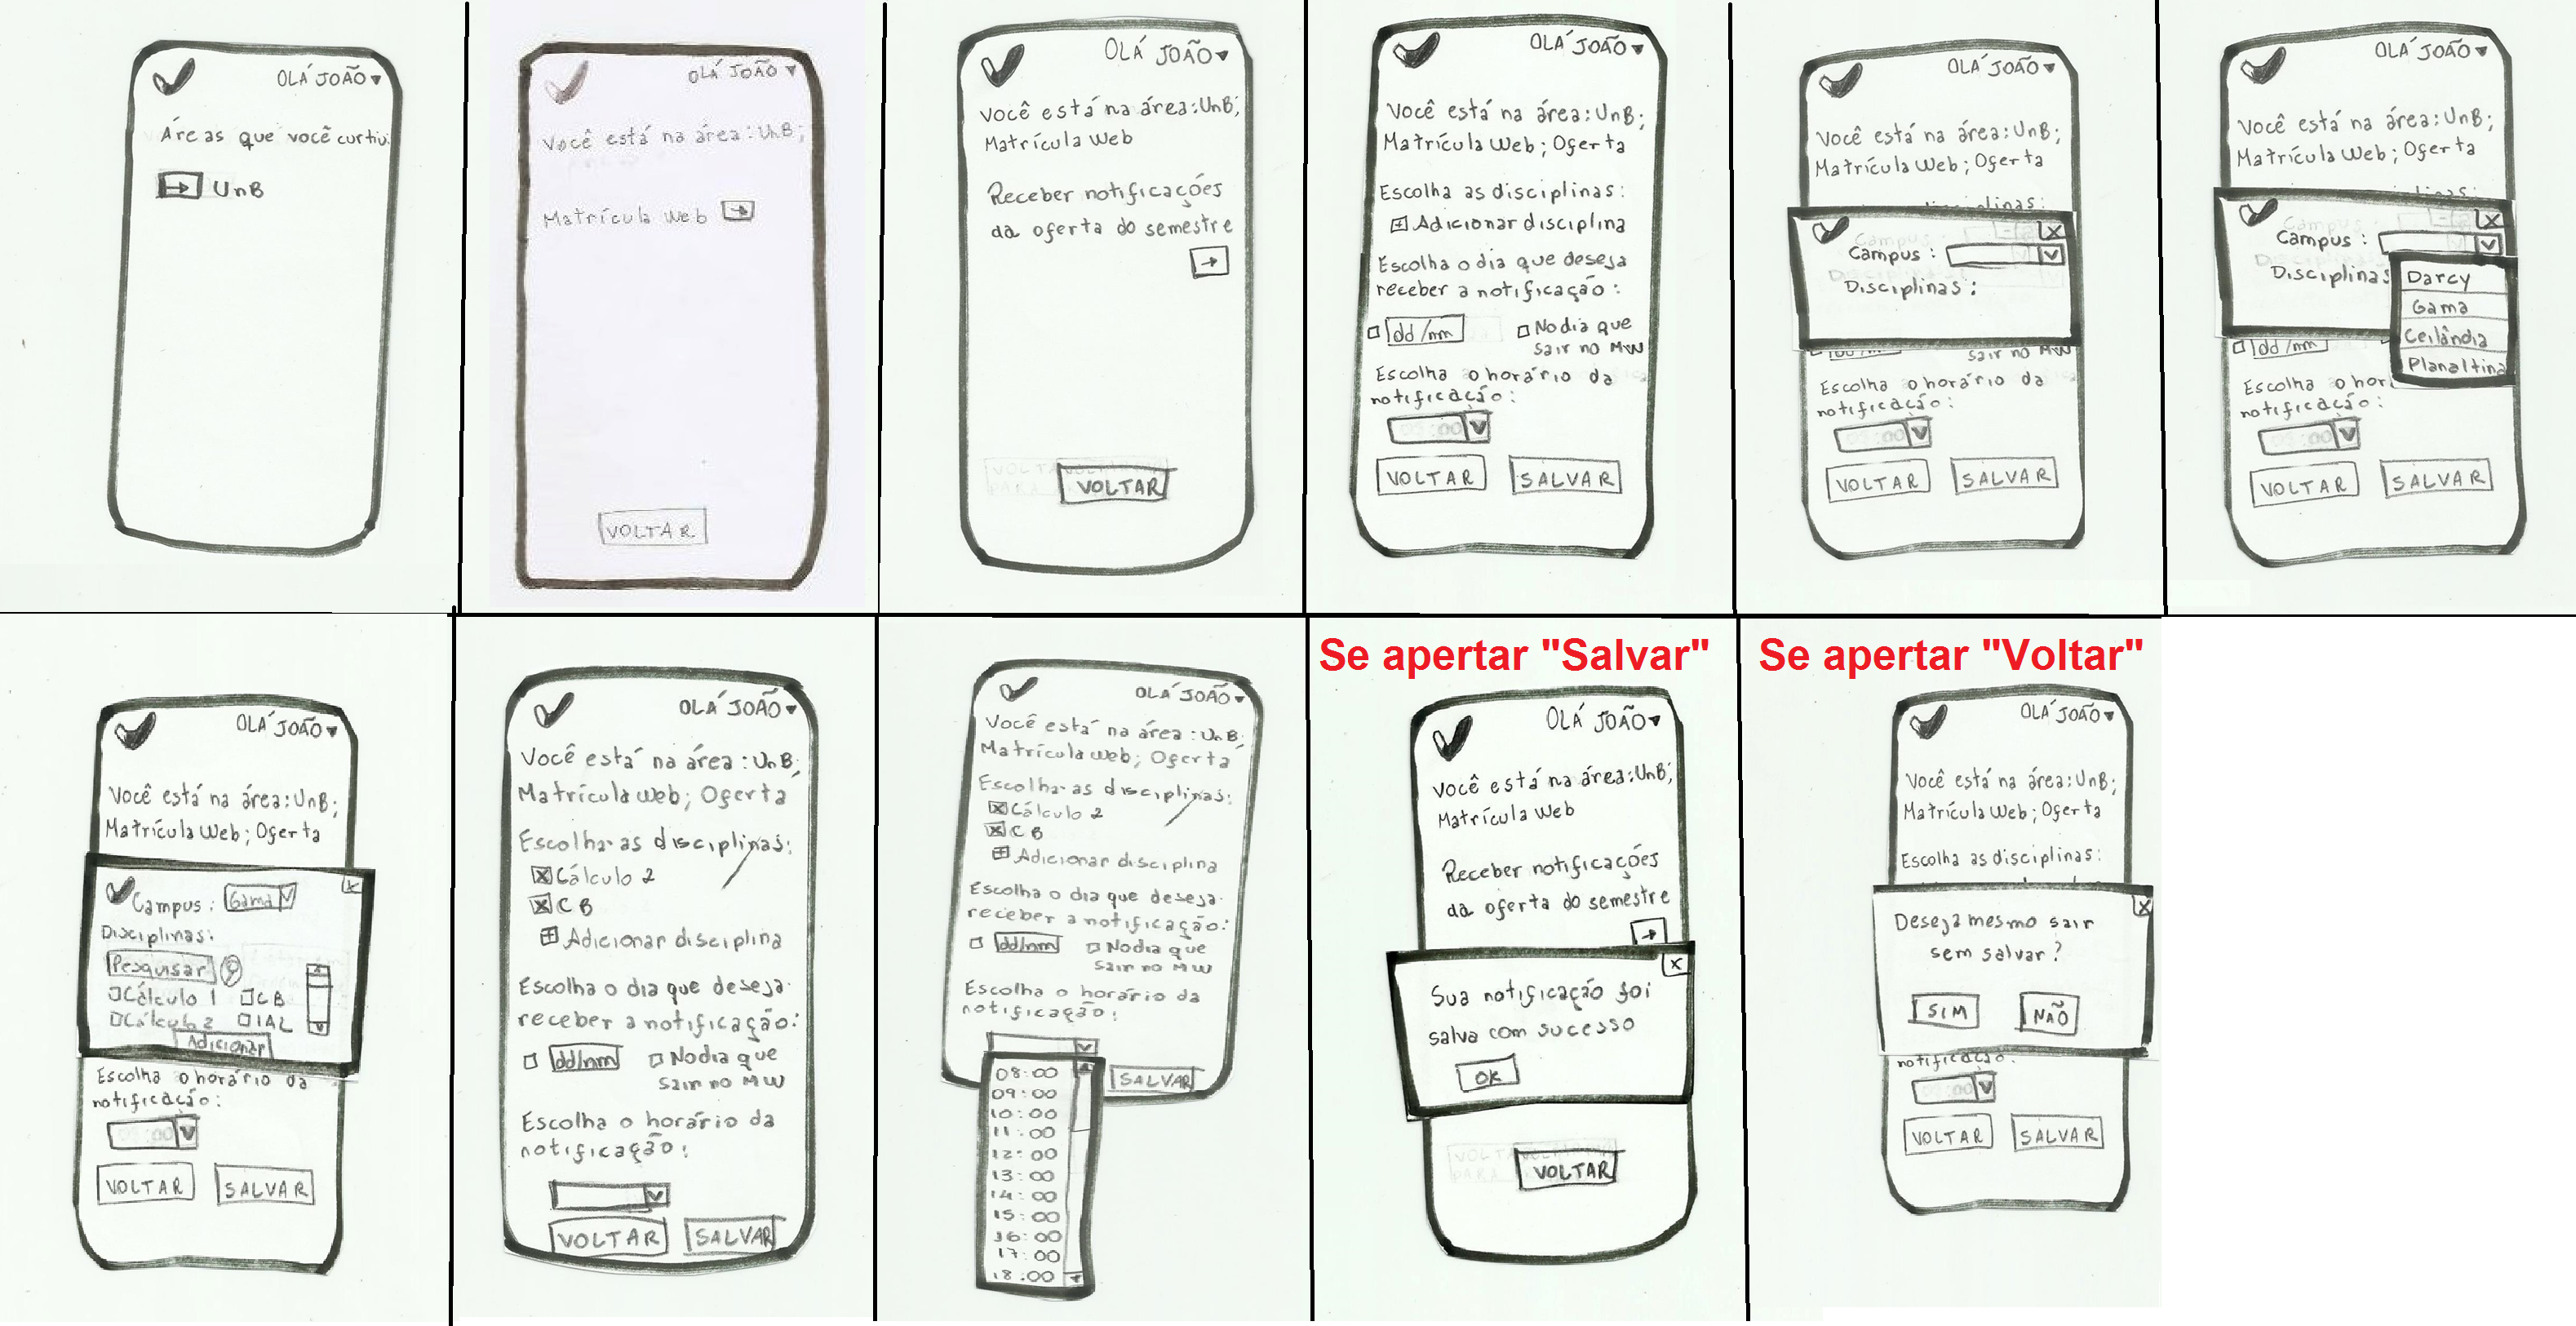
\includegraphics[width = 17.5cm, height = 15cm]{passos3}
 \caption{Protótipo de papel - Versão 3}
 \label{fig:passos2}

\end{figure}

\section{Protótipo na Ferramenta}
\label{mobile2}

\begin{figure}[h!]
  \centering
  \subfloat{
    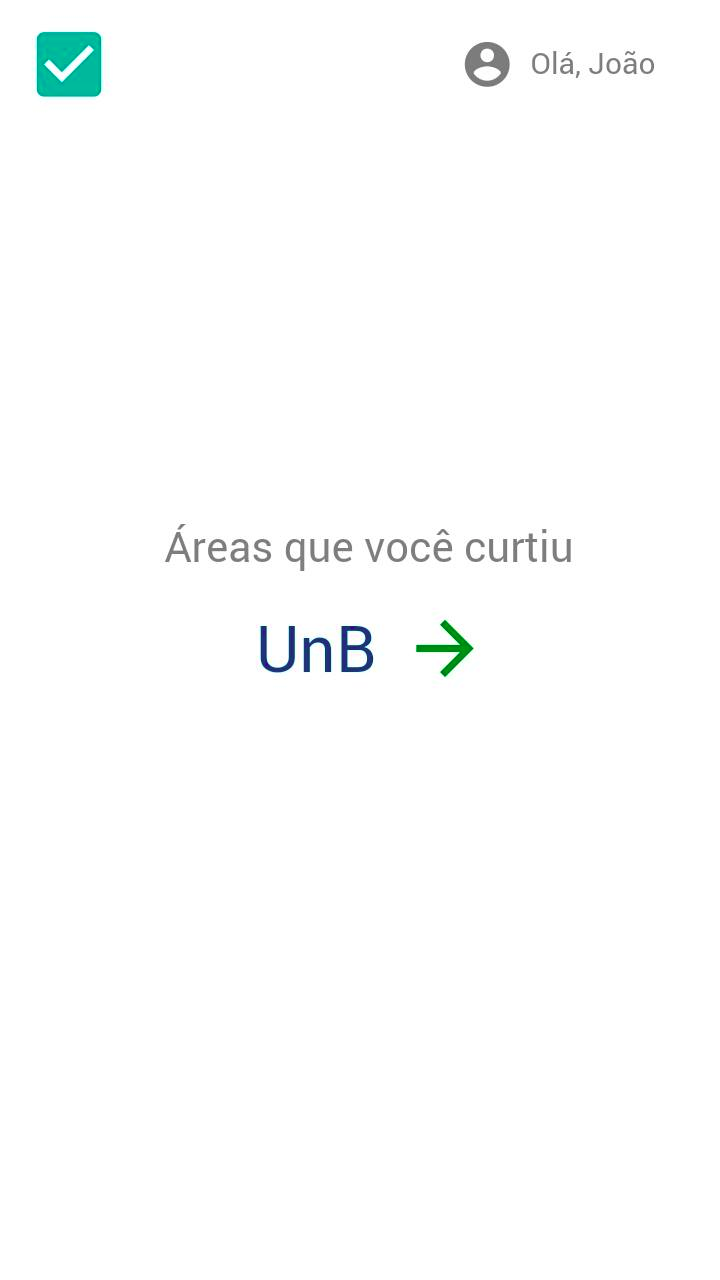
\includegraphics[keepaspectratio=true, scale=0.2]{figuras/mob11.png}
   }
   \subfloat{
      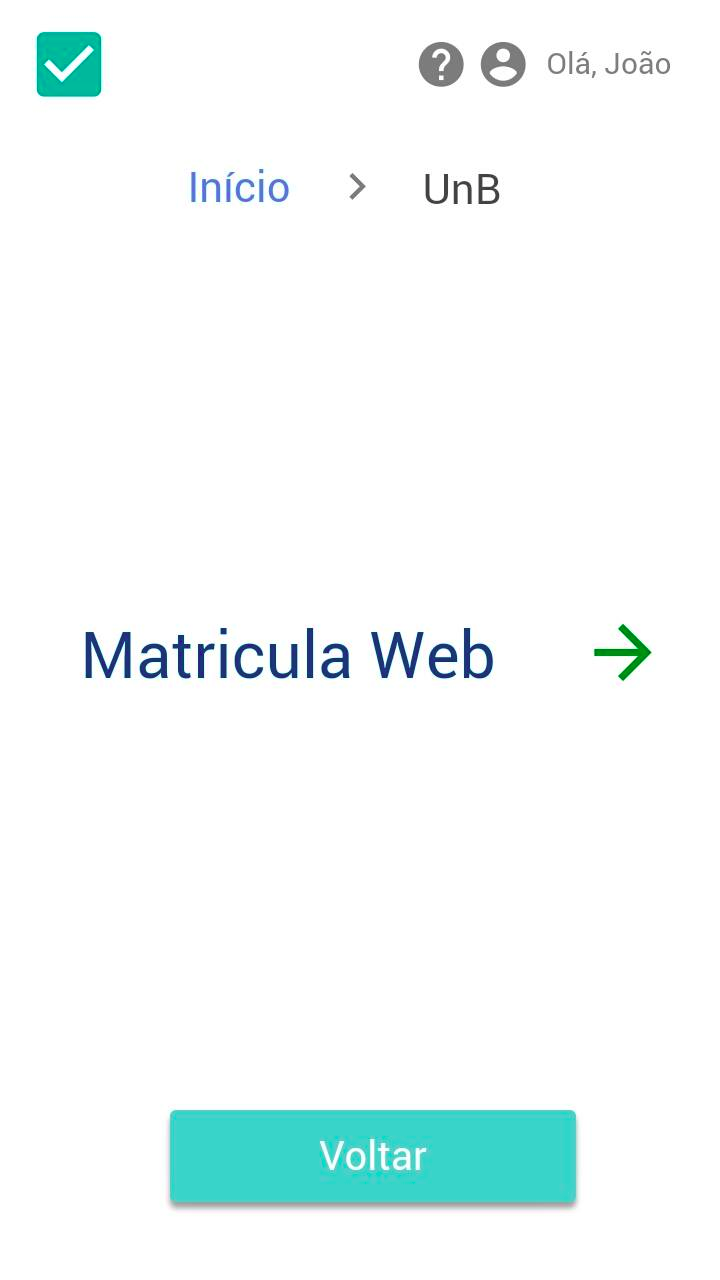
\includegraphics[keepaspectratio=true, scale=0.2]{figuras/mob12.png}
   }
    
\end{figure}

\begin{figure}[h!]
  \centering
  \subfloat{
    
\includegraphics[keepaspectratio=true, scale=0.2]{figuras/mob13.png}
   }
   \subfloat{
      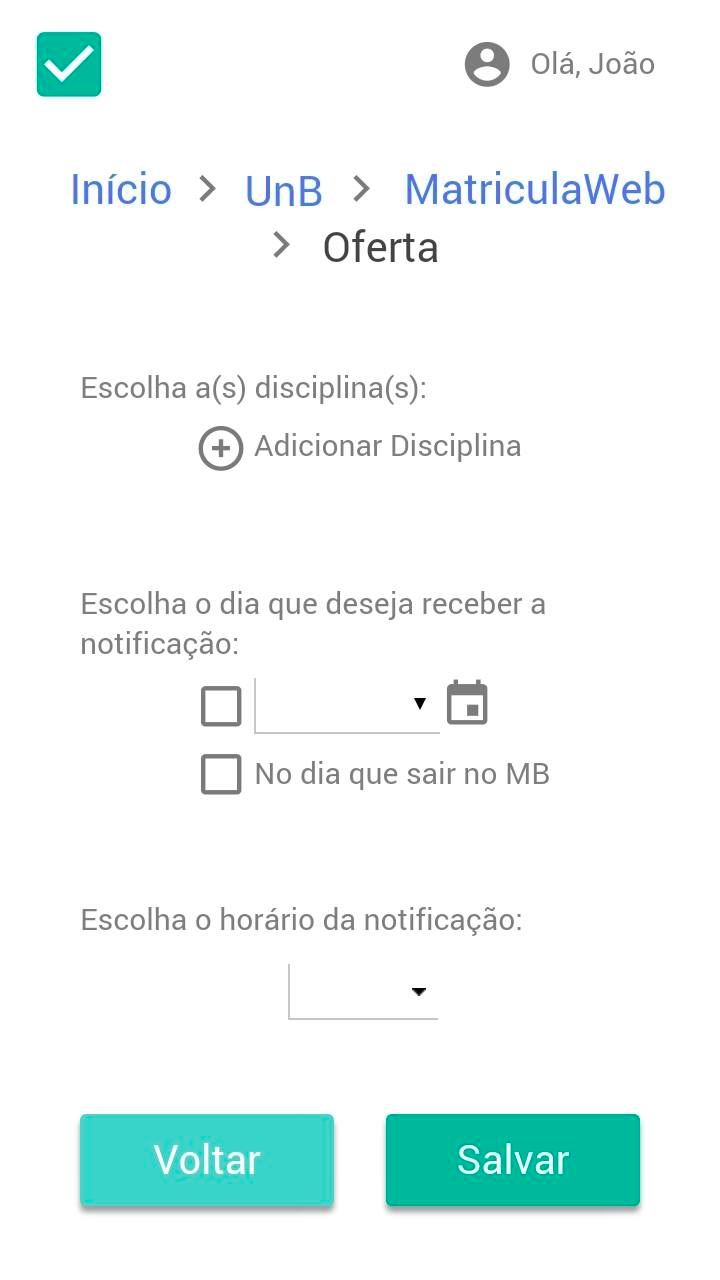
\includegraphics[keepaspectratio=true, scale=0.2]{figuras/mob14.png}
   }
    
\end{figure}

\begin{figure}[h!]
  \centering
  \subfloat{
    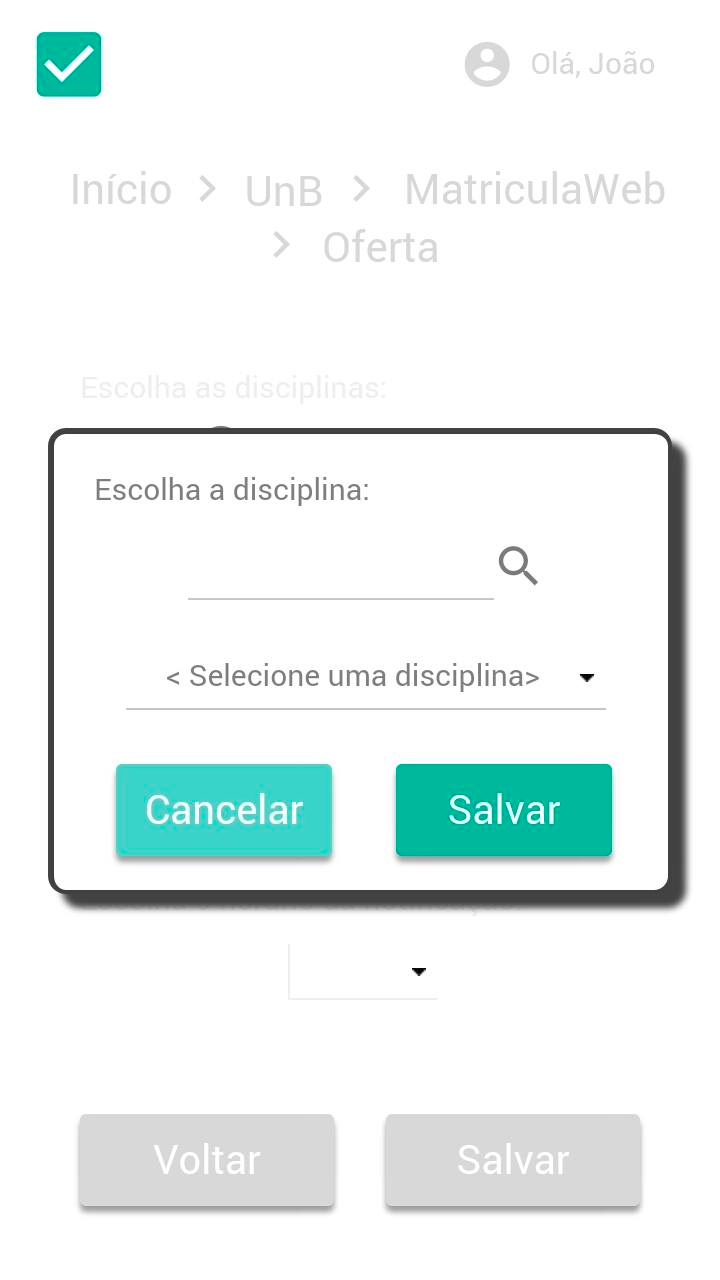
\includegraphics[keepaspectratio=true, scale=0.2]{figuras/mob15.png}
   }
   \subfloat{
      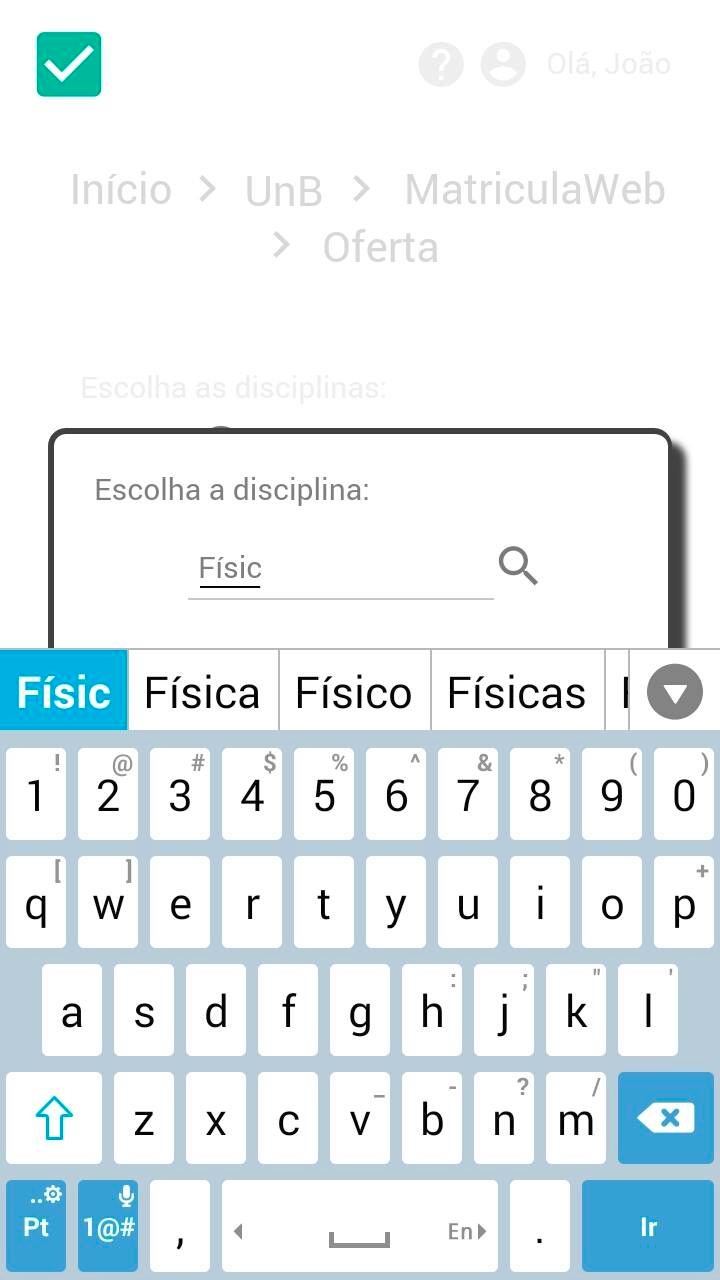
\includegraphics[keepaspectratio=true, scale=0.2]{figuras/mob25.png}
   }
    
\end{figure}

\begin{figure}[h!]
  \centering
  \subfloat{
    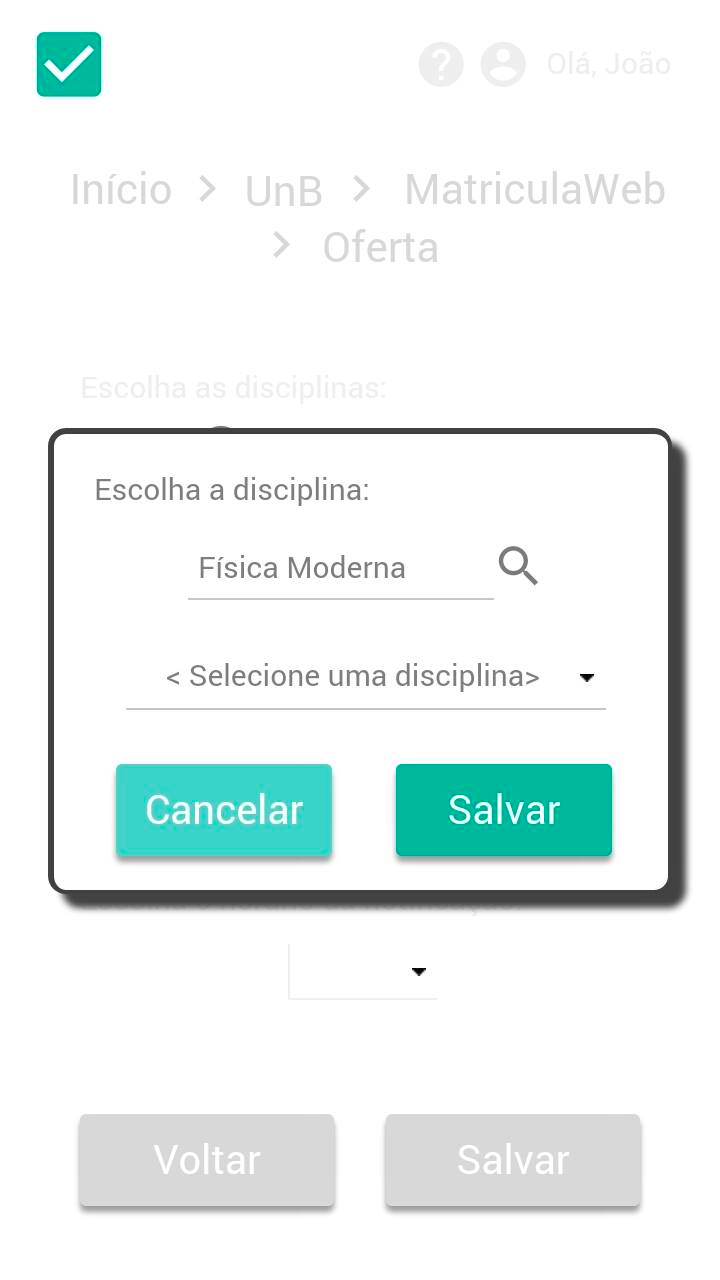
\includegraphics[keepaspectratio=true, scale=0.2]{figuras/mob251.png}
   }
   \subfloat{
      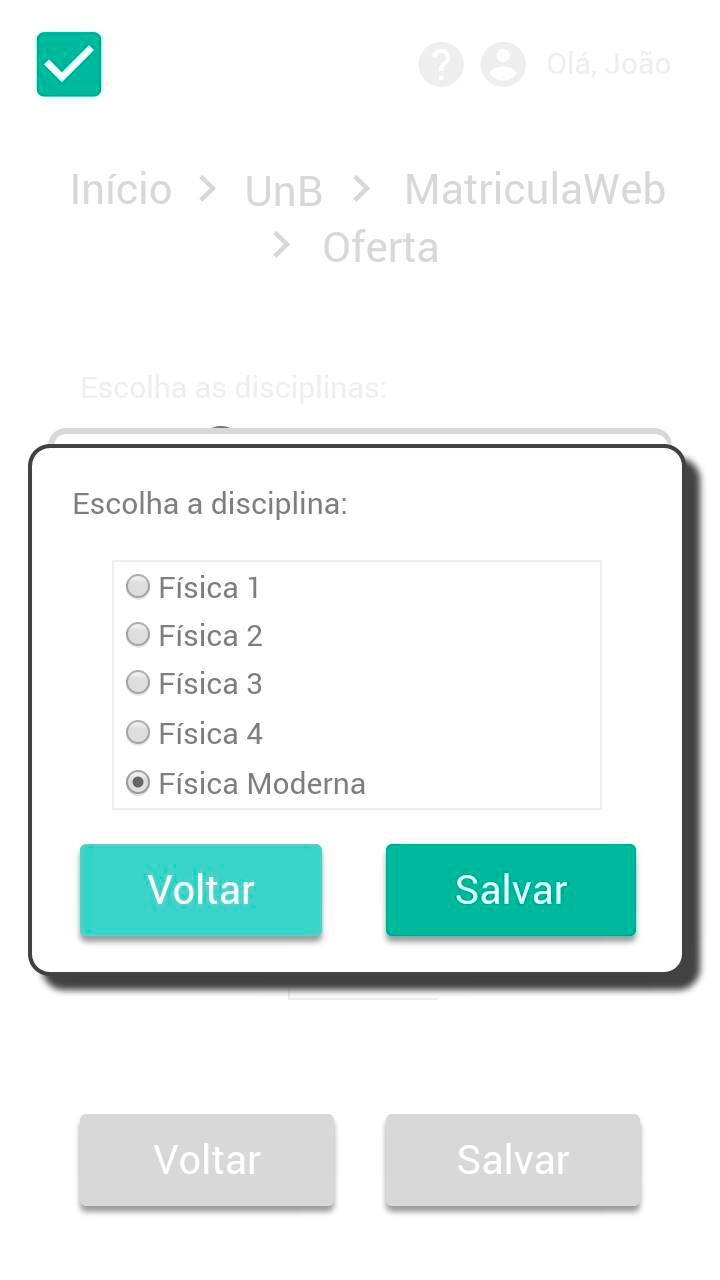
\includegraphics[keepaspectratio=true, scale=0.2]{figuras/mob26.png}
   }
    
\end{figure}

\begin{figure}[h!]
  \centering
  \subfloat{
    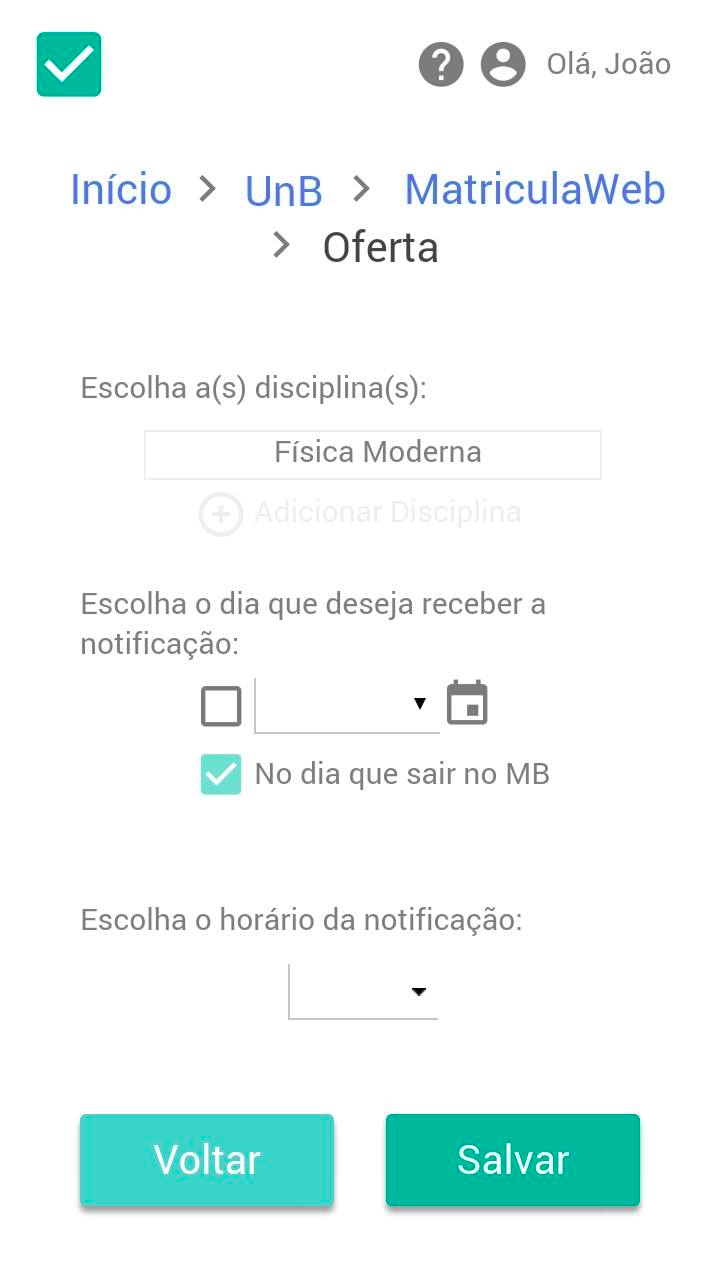
\includegraphics[keepaspectratio=true, scale=0.2]{figuras/mob27.png}
   }
   \subfloat{
      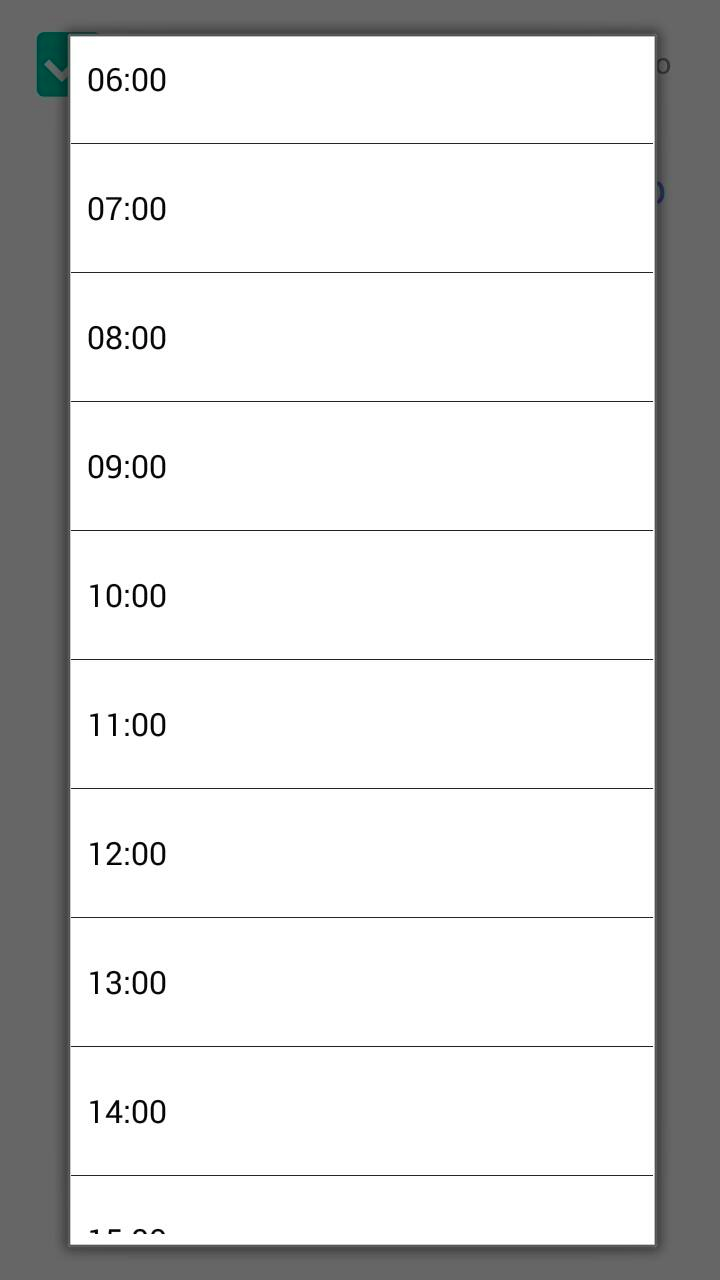
\includegraphics[keepaspectratio=true, scale=0.2]{figuras/mob28.png}
   }
    
\end{figure}

\begin{figure}[h!]
  \centering
  \subfloat{
    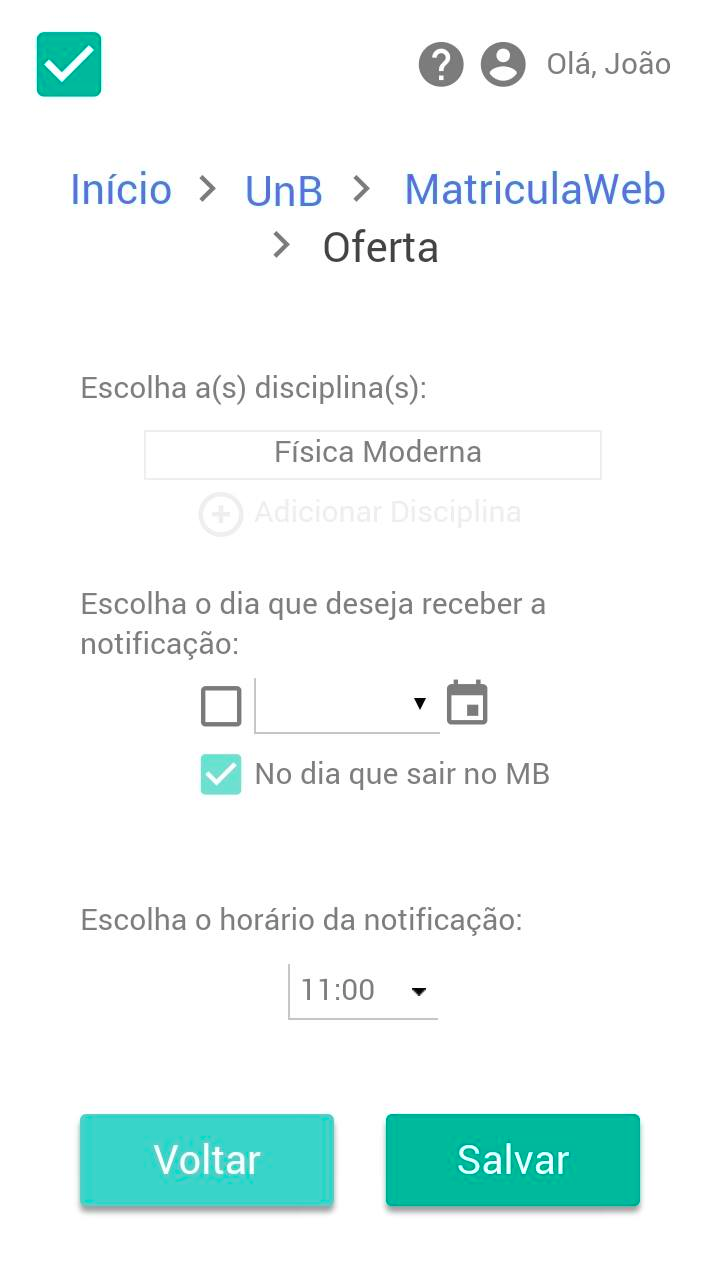
\includegraphics[keepaspectratio=true, scale=0.2]{figuras/mob29.png}
   }
   \subfloat{
      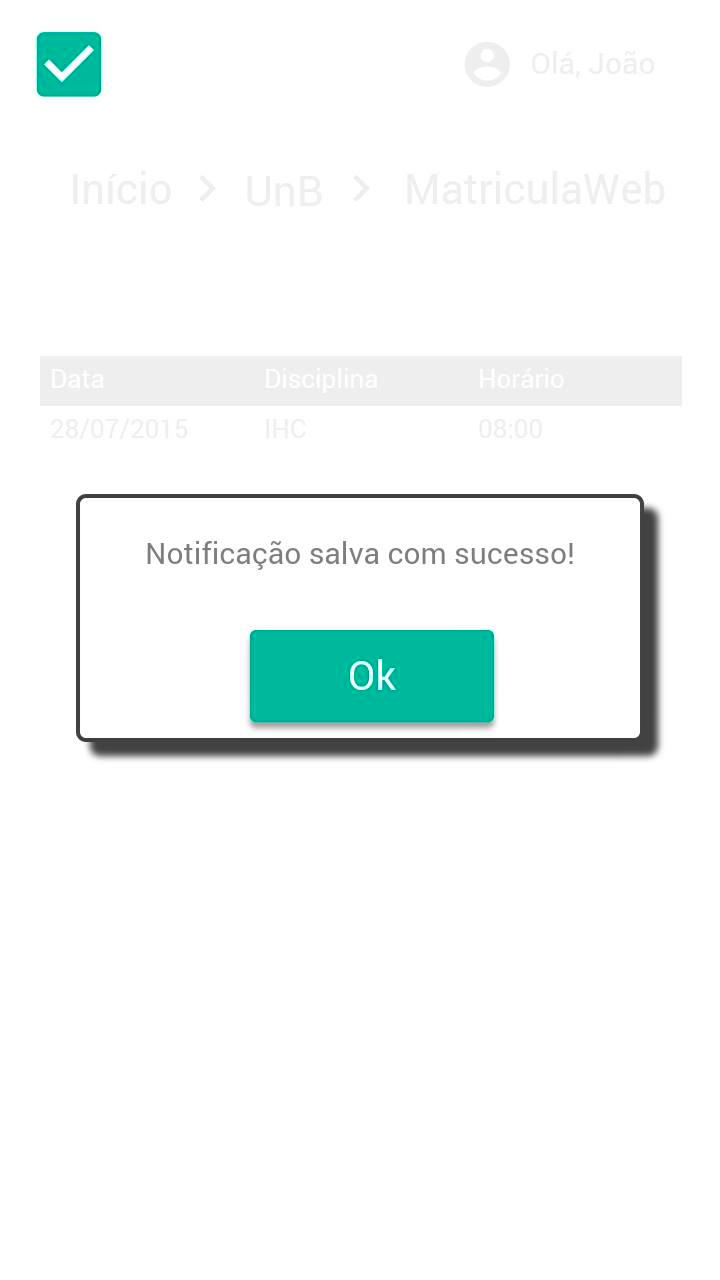
\includegraphics[keepaspectratio=true, scale=0.2]{figuras/mob115.png}
   }
    
\end{figure}

\begin{figure}[h!]
  \centering
   \subfloat{
      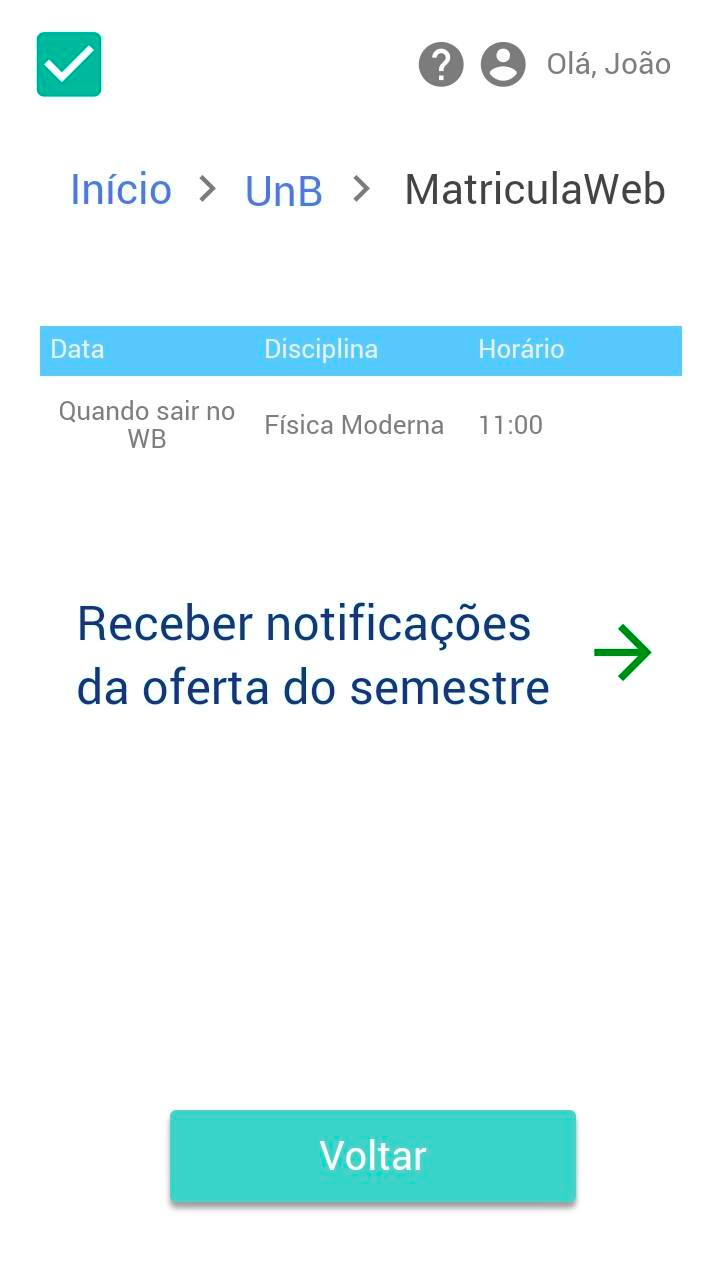
\includegraphics[keepaspectratio=true, scale=0.2]{figuras/mob216.png}
   }
\end{figure}

